\documentclass{beamer}

\usepackage[utf8x]{inputenc}
\usepackage{graphicx}
\usepackage{amsthm,amssymb,amsbsy,amsmath,amsfonts,amssymb,amscd}
\usepackage{dsfont}
\usepackage{array}
\newcolumntype{N}{@{}m{2pt}@{}}
\usepackage{tikz}
%\usetikzlibrary{arrows}
%\tikzstyle{block}=[draw opacity=0.7,line width=1.4cm]

\useoutertheme[subsection=false]{miniframes}
\usepackage{lmodern}

\setbeamercolor{author in head/foot}{fg=gray,bg=white}
\setbeamercolor{title in head/foot}{fg=gray,bg=white}
\setbeamercolor{page number in head/foot}{fg=gray,bg=white}
\setbeamercolor{section in head/foot}{bg=black,fg=gray}
\setbeamercolor{subsection in head/foot}{bg=black,fg=gray}

%%%%%%%%%%%%%%%%%%%%%%%%
% GENERAL BEAMER STYLE :

\setbeamertemplate{footline}{
  \hbox{%
    \begin{beamercolorbox}[wd=.2\paperwidth,ht=2ex,dp=1ex,left]{author in head/foot}%
      \hskip1em\usebeamerfont{author in head/foot}\insertshortauthor
    \end{beamercolorbox}%
    \begin{beamercolorbox}[wd=.7\paperwidth,ht=2ex,dp=1ex,center]{title in head/foot}%
      \usebeamerfont{title in head/foot}\insertshorttitle
    \end{beamercolorbox}%
    \begin{beamercolorbox}[wd=.1\paperwidth,ht=2ex,dp=1ex,right]{page number in head/foot}%
      \usebeamerfont{page number in head/foot}\insertframenumber{} / \inserttotalframenumber
      \kern1em 
    \end{beamercolorbox}
  }
}

\setbeamercolor{alerted text}{fg=red!80!black}
\setbeamercolor{itemize/enumerate subbody}{fg=gray!70!black}
\setbeamertemplate{itemize item}[square]
\setbeamertemplate{itemize subitem}[triangle]%{{\textendash}}
\setbeamerfont{itemize/enumerate subbody}{size=\footnotesize}
\setbeamerfont{itemize/enumerate subitem}{size=\footnotesize}

\setbeamertemplate{navigation symbols}{}

\AtBeginSection{
\begin{frame}
    \begin{centering}
    \begin{beamercolorbox}[sep=12pt,center]{part title}
    \usebeamerfont{section title}\insertsection\par
    \end{beamercolorbox}
    \end{centering}
\end{frame}
}

 


\title[Majeure Data Science -- Surrogate models and GPR]{\texorpdfstring{ \small Surrogate models and Gaussian Process regression -- lecture 5/5 \\ \vspace{3mm} \LARGE Advanced GPR}{}}
\author[Mines St-\'Etienne ]{Mines St-\'Etienne -- Majeure Data Science -- 2016/2017}
\institute{\texorpdfstring{Nicolas Durrande (durrande@emse.fr)}{}}
\date{\null}

\DeclareMathOperator*{\Var}{var}
\DeclareMathOperator*{\E}{E}
\DeclareMathOperator*{\Cov}{cov}
\newcommand\PR[1]{\mathrm{P}\left(#1 \right)}
\newcommand\PS[1]{{\langle #1 \rangle}_\mathcal{H}}
\newcommand\PSi[2]{{ \left \langle #1 \right \rangle}_{\! #2}}
\newcommand\N[2]{{|| #1 ||}_{\! #2}}
\newcommand\dx{\, \mathrm{d}}
\newcommand\textequal{\rule[.4ex]{4pt}{0.4pt}\llap{\rule[.7ex]{4pt}{0.4pt}}}
\newcommand{\argmin}{\operatornamewithlimits{argmin}}
\makeatletter
\newcommand{\shorteq}{%
  \settowidth{\@tempdima}{a}% Width of hyphen
  \resizebox{\@tempdima}{\height}{=}%
}
\makeatother

\newenvironment{psmallmatrix}
  {\left(\begin{smallmatrix}}
  {\end{smallmatrix}\right)}


%%%%%%%%%%%%%%%%%%%%%%%%%%%%%%%%%%%%%%%%%%%%%%%%%%%%%%
%%%%%%%%%%%%%%%%%%%%%%%%%%%%%%%%%%%%%%%%%%%%%%%%%%%%%%
%%%%%%%%%%%%%%%%%%%%%%%%%%%%%%%%%%%%%%%%%%%%%%%%%%%%%%
\begin{document}
\setbeamercolor{author in head/foot}{fg=gray,bg=white}
\setbeamercolor{title in head/foot}{fg=gray,bg=white}
\setbeamercolor{page number in head/foot}{fg=gray,bg=white}
\setbeamercolor{section in head/foot}{bg=black,fg=gray}
\setbeamercolor{subsection in head/foot}{bg=black,fg=gray}

%%%%%%%%%%%%%%%%%%%%%%%%%%%%%%%%%%%%%%%%%%%%%%%%%%%%%%
\begin{frame}
  \titlepage
\end{frame}

%%%%%%%%%%%%%%%%%%%%%%%%%%%%%%%%%%%%%%%%%%%%%%%%%%%%%%
%%%%%%%%%%%%%%%%%%%%%%%%%%%%%%%%%%%%%%%%%%%%%%%%%%%%%%
\section[Multioutputs GPR]{Multioutputs GPR / GPR with categorical inputs}
\subsection{}

%%%%%%%%%%%%%%%%%%%%%%%%%%%%%%%%%%%%%%%%%%%%%%%%%%%%%%
\begin{frame}{}
\begin{exampleblock}{Example}
	We observe the temperature in two cities $A$ and $B$ for a few time points $X_A$ and $X_B$. We assume a Gaussian process prior for these $T_A(t)$ and $T_B(t)$. What would be your prediction for the temperature in $A$ at a new time point $t$?
\end{exampleblock}
\pause
Ideally, we are interested in $T_A(t)|T_A(X_A), T_B(X_B)$. If $(T_A(t),\ T_A(X_A),\ T_B(X_B))$ is a Gaussian vector, we know how to compute the conditional distribution. However, it requires the cross covariance $k_{AB}(t,t') = \Cov[T_A(t),T_B(t')]$.
\end{frame}

%%%%%%%%%%%%%%%%%%%%%%%%%%%%%%%%%%%%%%%%%%%%%%%%%%%%%%
\begin{frame}{}
\begin{exampleblock}{Exercise}
Compute the distribution of $T_A(t)|T_A(X_A), T_B(X_B)$.
\end{exampleblock}
\pause
\begin{exampleblock}{Solution}
\vspace{2mm}
The conditional mean is:
\small
\begin{equation*}
	\begin{split}
		m_A(t) &= \E[T_A(t)|T_A(X_A) \shorteq F_A, T_B(X_B) \shorteq F_B] \\
		& \begin{pmatrix}
			k_A(t,X_A) & k_{AB}(t,X_B)
		\end{pmatrix}
		\begin{pmatrix}
			k_A(X_A,X_A) & k_{AB}(X_A,X_B) \\
			k_{AB}(X_A,X_B)^t & k_{B}(X_B,X_B) \\
		\end{pmatrix}^{-1}
		\begin{pmatrix}
			F_A \\
			F_B \\
		\end{pmatrix}
	\end{split}
\end{equation*}
\normalsize
The conditional covariance is:
\small
\begin{equation*}
	\begin{split}
		c_A(t,t') &=  \Cov[T_A(t),T_A(t')|T_A(X_A) \shorteq F_A, T_B(X_B) \shorteq F_B] \\
		&= k_A(t,t') - 
		\begin{pmatrix}
			k_A(t,X_A) & k_{AB}(t,X_B)
		\end{pmatrix} \\
		&  \hspace{2.5cm} \times
		\begin{pmatrix}
			k_A(X_A,X_A) & k_{AB}(X_A,X_B) \\
			k_{AB}(X_A,X_B)^t & k_{B}(X_B,X_B) \\
		\end{pmatrix}^{-1}
		\begin{pmatrix}
			k_A(t',X_A)^t \\
			k_{AB}(t',X_B)^t
		\end{pmatrix}
	\end{split}
	%\label{eq:multiGPR}
\end{equation*}
\end{exampleblock}
\end{frame}

%%%%%%%%%%%%%%%%%%%%%%%%%%%%%%%%%%%%%%%%%%%%%%%%%%%%%%
\begin{frame}{}
\begin{example}
	If we do the same thing fot $T_B$ we obtain:
	\begin{center}
	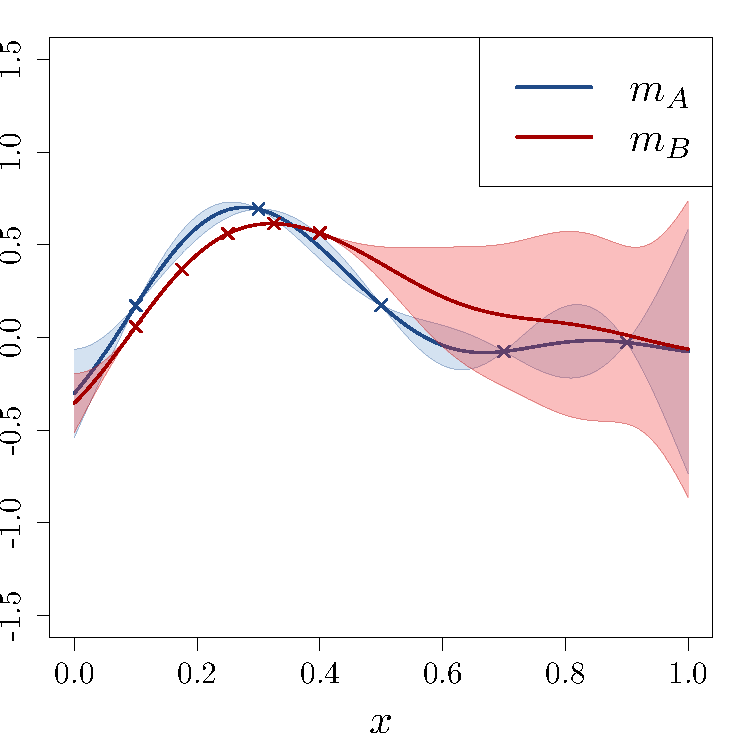
\includegraphics[height=7cm]{figures/R/ch2_multiGPR1}
	\end{center}
\end{example}
\end{frame}

%%%%%%%%%%%%%%%%%%%%%%%%%%%%%%%%%%%%%%%%%%%%%%%%%%%%%%
\begin{frame}{}
Instead of considering the GP to be multioutput, it is possible to see the GP as having one input but one extra categorical variable:
\begin{equation*}
 Z(t,c) = 
 \begin{cases}
   Z_A(t) & \text{if } c=A	\\
   Z_B(t) & \text{if } c=B.	
 \end{cases}
\end{equation*}
\begin{exampleblock}{Exercise:}
	Compute the kernel of $Z$.
\end{exampleblock}
\vspace{3mm}
With this settings, the conditional mean
\small
\begin{equation*}
	\begin{split}
		m_A(t) &= 
		 \begin{pmatrix}
			k_A(t,X_A) & k_{AB}(t,X_B)
		\end{pmatrix}
		\begin{pmatrix}
			k_A(X_A,X_A) & k_{AB}(X_A,X_B) \\
			k_{AB}(X_A,X_B)^t & k_{B}(X_B,X_B) \\
		\end{pmatrix}^{-1}
		\begin{pmatrix}
			F_A \\
			F_B \\
		\end{pmatrix}
	\end{split}
\end{equation*}
\normalsize
writes as an usual conditional mean
\small
\begin{equation*}
	\begin{split}
		m_A(t) = m(t,A) = \E[T(t,A)|T(X) \shorteq F] = 
		k(\begin{psmallmatrix} t \\ A \end{psmallmatrix},X) k(X,X)^{-1} F
	\end{split}
\end{equation*}
\normalsize
\end{frame}


%%%%%%%%%%%%%%%%%%%%%%%%%%%%%%%%%%%%%%%%%%%%%%%%%%%%%%
\begin{frame}{}
\begin{example}
	We obtain this representation for the model
	\begin{center}
	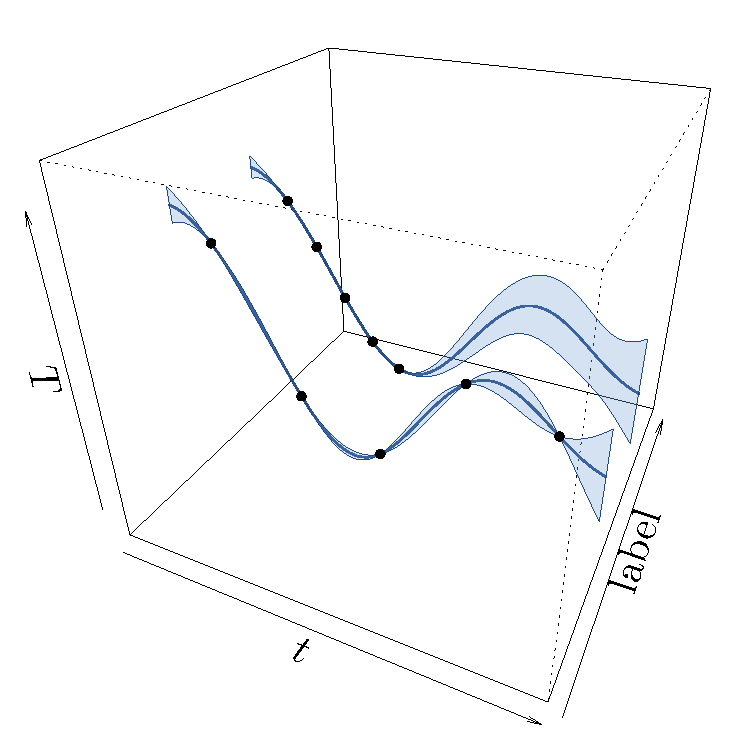
\includegraphics[height=7cm]{figures/R/ch2_multiGPR}
	\end{center}
\end{example}
\end{frame}


%%%%%%%%%%%%%%%%%%%%%%%%%%%%%%%%%%%%%%%%%%%%%%%%%%%%%%
\begin{frame}{}
In the end, multioutputs GPs can be seen as GPs with one extra categorical variable indicating the output label.\\
\vspace{5mm}
All the math stay the same, we just need to specify a covariance function that takes into account this extra variable. A common approach is to consider a product covariance structure
\begin{equation*}
k\left( \begin{psmallmatrix} \phantom{'}t\phantom{'} \\ \phantom{'}c\phantom{'} \end{psmallmatrix},\begin{psmallmatrix} t' \\ c' \end{psmallmatrix} \right) = k_{cont}(t,t') k_{disc}(c,c')
\end{equation*}
where $k_{disc}(c,c')$ can be described by a covariance matrix. In practice, this covariance matrix has to be estimated. If there are to outputs (or two levels for the categorical variable), it is a $2 \ times 2$ covariance matrix. It can be parameterised by
\small
$$k_{disc} = 
\begin{pmatrix}
	\sigma_1^2 & \sigma_1 \sigma_2 \rho \\
	\sigma_1 \sigma_2 \rho & \sigma_2^2 \\
\end{pmatrix}$$
\normalsize
with  $\sigma_1,\ \sigma_2 \geq 0$ and $\rho \in [-1,1]$. The latter can be estimated by ML.
\vspace{5mm}

\end{frame}

%%%%%%%%%%%%%%%%%%%%%%%%%%%%%%%%%%%%%%%%%%%%%%%%%%%%%%
\begin{frame}{}
In higher dimension, it is possible to consider the following parameterization for $k_{disc}$:
\small
$$k_{disc} = W W^T$$
\normalsize
with  $\sigma_1,\ \sigma_2 \geq 0$ and $\rho \in [-1,1]$.
\vspace{5mm}

\end{frame}

%%%%%%%%%%%%%%%%%%%%%%%%%%%%%%%%%%%%%%%%%%%%%%%%%%%%%%
\begin{frame}{}
With this framework, the conditioning can also include observations more sophisticated than $Z(X)=F$... \\
\vspace{5mm}
For instance, if we know the integral of the function to approximate and it's derivative in a few points, we want to consider
$$ Z \ \left| \ Z(X) = F, \int Z = a, \frac{\dx Z}{\dx x}(X')= F' \right. $$
\end{frame}

%%%%%%%%%%%%%%%%%%%%%%%%%%%%%%%%%%%%%%%%%%%%%%%%%%%%%%
\begin{frame}{}
\begin{example}
	If we take into account that the function is centred, we obtain:
	\begin{center}
	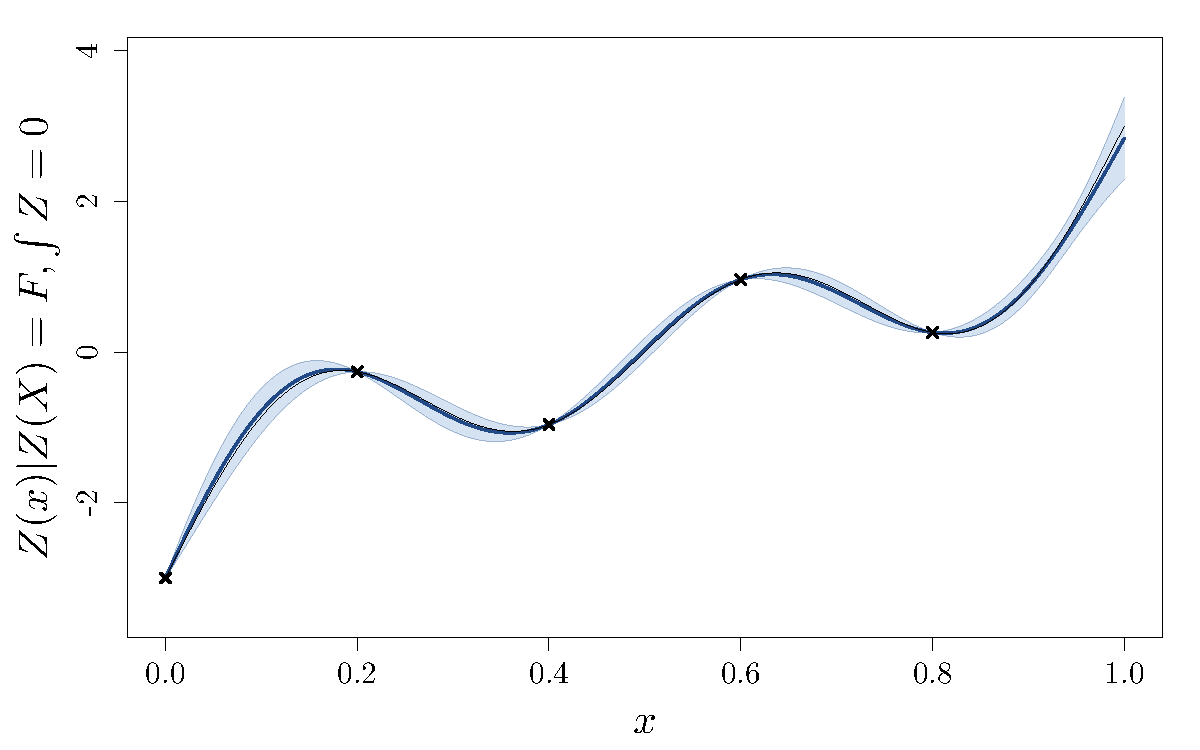
\includegraphics[height=6cm]{figures/R/exotic_int}
	\end{center}
\end{example}
\end{frame}

%%%%%%%%%%%%%%%%%%%%%%%%%%%%%%%%%%%%%%%%%%%%%%%%%%%%%%
\begin{frame}{}
\begin{example}
	Whereas if we ignore it:
	\begin{center}
	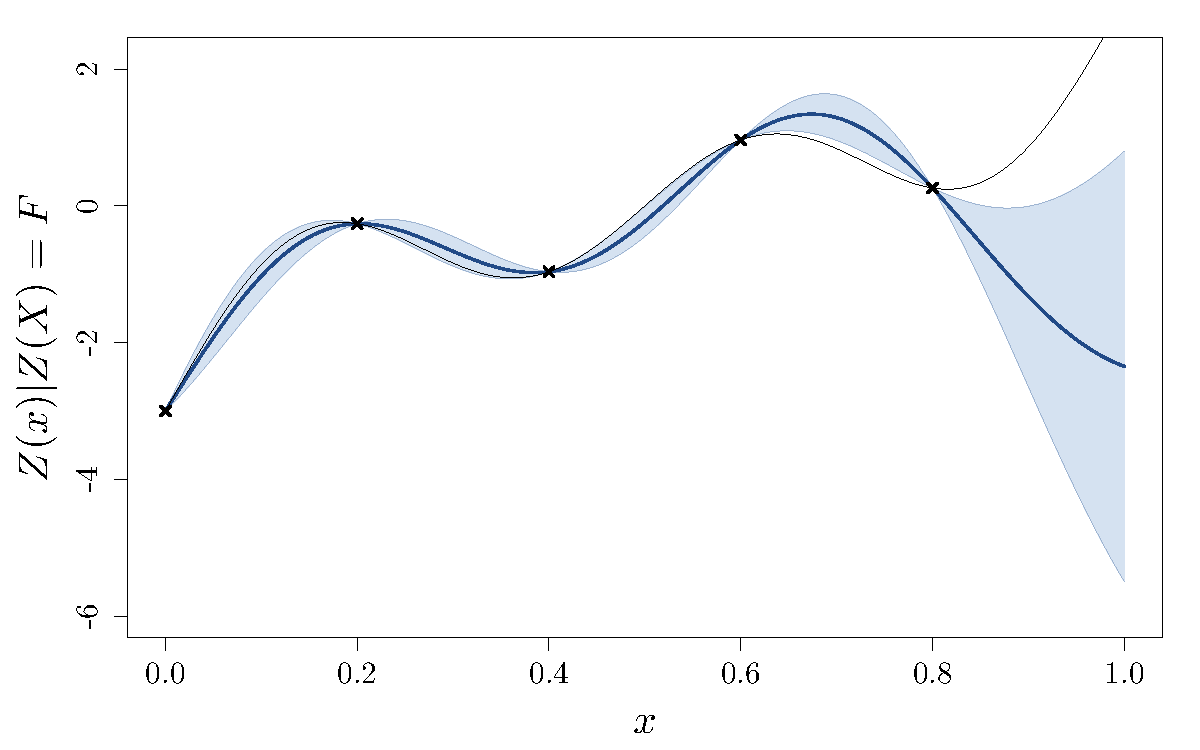
\includegraphics[height=6cm]{figures/R/exotic_pasint}
	\end{center}
\end{example}
\end{frame}

%%%%%%%%%%%%%%%%%%%%%%%%%%%%%%%%%%%%%%%%%%%%%%%%%%%%%%
\begin{frame}{}
Similarly, we can include in the model some derivative observations:
	\begin{center}
	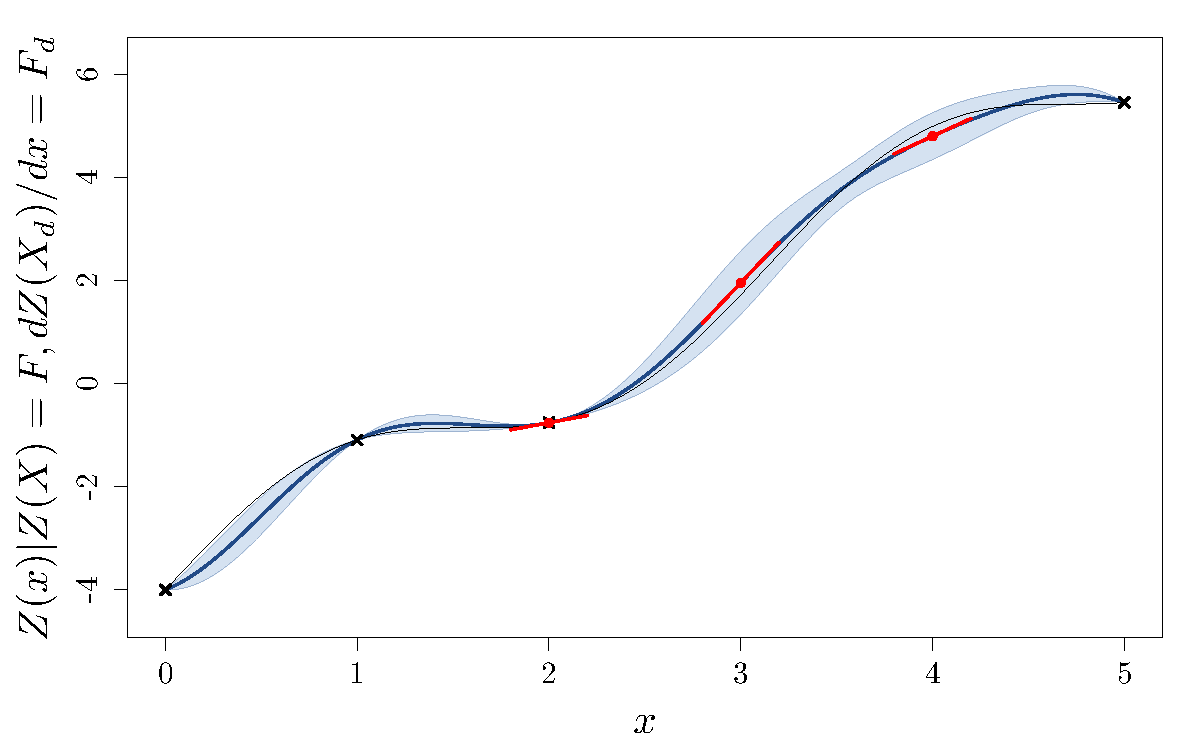
\includegraphics[height=6cm]{figures/R/exotic_der}
	\end{center}
\end{frame}

%%%%%%%%%%%%%%%%%%%%%%%%%%%%%%%%%%%%%%%%%%%%%%%%%%%%%%
\begin{frame}{}
We can see interesting behaviour if we look at a model with only derivatives.
	\begin{center}
	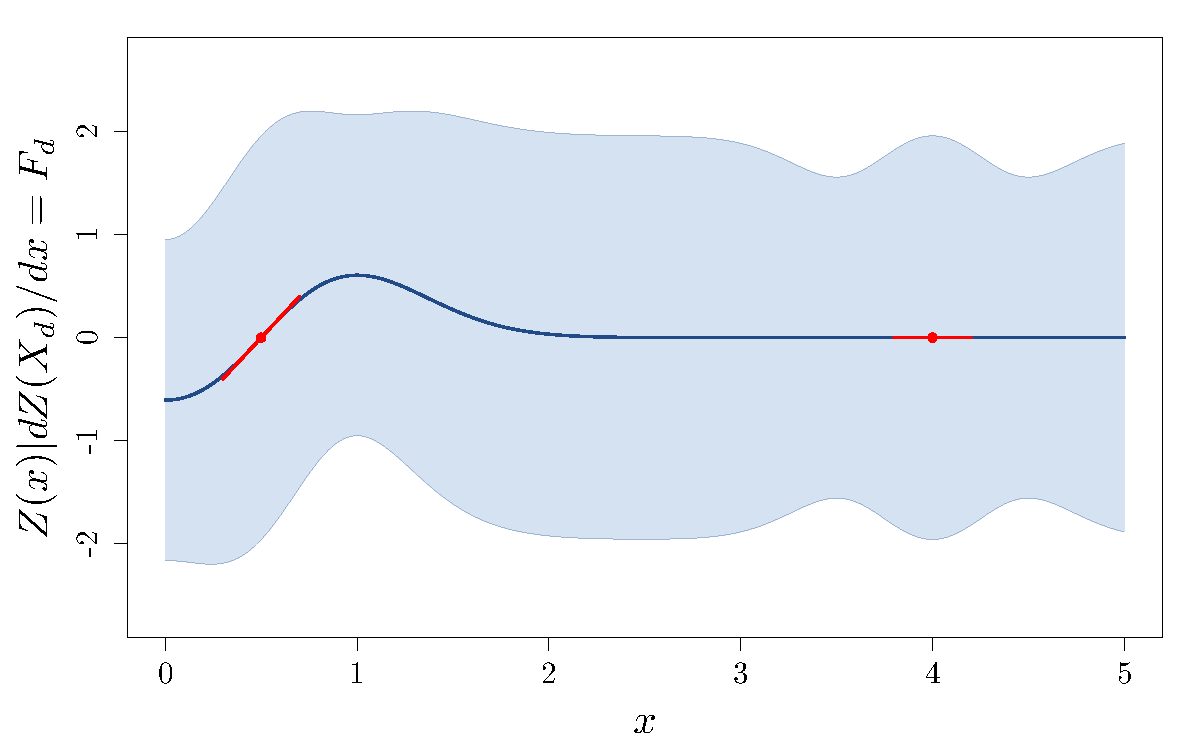
\includegraphics[height=6cm]{figures/R/exotic_deronly}
	\end{center}
\end{frame}

%%%%%%%%%%%%%%%%%%%%%%%%%%%%%%%%%%%%%%%%%%%%%%%%%%%%%%
\begin{frame}{}
As always, we can simulate conditional paths:
	\begin{center}
	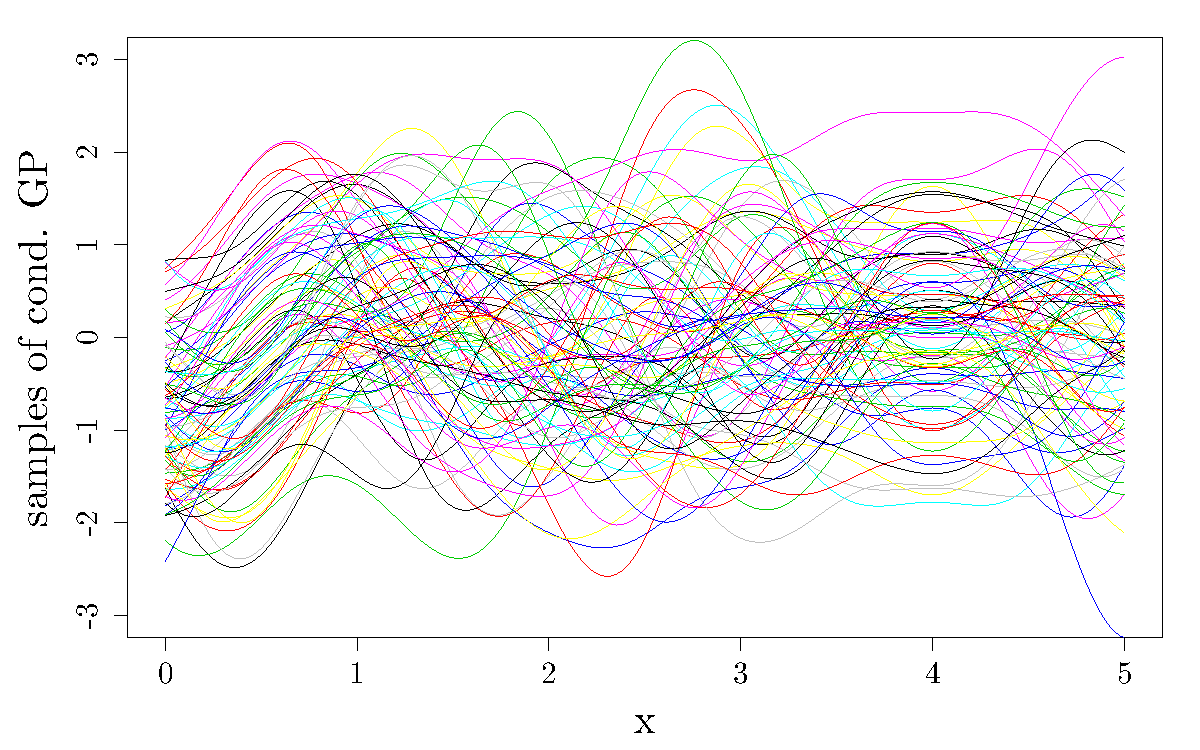
\includegraphics[height=6cm]{figures/R/exotic_simul}
	\end{center}
\end{frame}

%%%%%%%%%%%%%%%%%%%%%%%%%%%%%%%%%%%%%%%%%%%%%%%%%%%%%%
%%%%%%%%%%%%%%%%%%%%%%%%%%%%%%%%%%%%%%%%%%%%%%%%%%%%%%
\section{Conclusion}
\subsection{}

%%%%%%%%%%%%%%%%%%%%%%%%%%%%%%%%%%%%%%%%%%%%%%%%%%%%%%
\begin{frame}{}
\begin{block}{Small Recap}
\begin{itemize}
 \item GPR models do not necessarily interpolate. \vspace{2mm}
 \item Multi-output GPR is straightforward
 \item Various way to create new kernels:
 \begin{itemize}
 	\item Finite dim kernels
 	\item Bochner theorem
 	\item Making New from Old
 	\item Linear operators
 \end{itemize}
\end{itemize}
\end{block}

\begin{block}{Making new from old}
\begin{itemize}
 \item sum
 \item product
 \item kernel rescaling
\end{itemize}
\end{block}
\end{frame}



\end{document}
%%%%%%%%%%%%%%%%%%%%%%%%%%%%%%%%%%%%%%%%%%%%%%%%%%%%%%%%%%%%%%%%%%%%%%%%%%%%%%%
%%%%%%%%%%%%%%%%%%%%%%%%%%%%%%%%%%%%%%%%%%%%%%%%%%%%%%%%%%%%%%%%%%%%%%%%%%%%%%%
%%%%%%%%%%%%%%%%%%%%%%%%%%%%%%%%%%%%%%%%%%%%%%%%%%%%%%%%%%%%%%%%%%%%%%%%%%%%%%%
%%%%%%%%%%%%%%%%%%%%%%%%%%%%%%%%%%%%%%%%%%%%%%%%%%%%%%%%%%%%%%%%%%%%%%%%%%%%%%%



\structure{}

\begin{center}
  \begin{tabular}{|c|cc|}

  \end{tabular}
\end{center}

###
%%%%%%%%%%%%%%%%%%%%%%%%%%%%%%%%%%%%%%%%%%%%%%%%%%%%%%
\begin{frame}{}

\end{frame}

###
\begin{block}{}

\end{block}

###
\begin{center}
\includegraphics[height=5cm]{figures/}
\end{center}

###
\begin{columns}[c]
\column{5cm}

\column{5cm}

\end{columns}
